% Final report, 17-739/18-739 (Fall 2026). Compile on Overleaf (pdfLaTeX + BibTeX): upload the whole report/ folder.
% Section owners (report/OUTLINE.md): Prisca = abstract, 1, 3, 4, 5.2-5.4, 9 · Eileen = 2, 5.1 (protocol), 6 · both = 7, 8.
\documentclass[conference]{IEEEtran}
\usepackage[utf8]{inputenc}
\usepackage[T1]{fontenc}
\usepackage{amsmath}
\usepackage{booktabs}
\usepackage{multirow}
\usepackage{graphicx}
\usepackage{xcolor}
\usepackage{listings}
\usepackage{tikz}
\usetikzlibrary{positioning,arrows.meta}
\usepackage{cite}
\usepackage[hidelinks]{hyperref}

\lstset{basicstyle=\ttfamily\scriptsize, columns=fullflexible, breaklines=true, frame=single,
        framerule=0.3pt, xleftmargin=2pt, xrightmargin=2pt, showstringspaces=false}
\newcommand{\todo}[1]{\textcolor{red}{[TODO: #1]}}
\newcommand{\safe}{\textsc{safe}}
\newcommand{\vuln}{\textsc{vulnerable}}

\begin{document}

\title{Fooling the Copilot: Code Changes Don't Make an LLM Miss a Bug,\\ but Trusting Code It Can't See Does}

% TODO (Prisca): confirm full names and how you want to be listed.
\author{\IEEEauthorblockN{Prisca \todo{surname} \quad Eileen \todo{surname}}
\IEEEauthorblockA{Carnegie Mellon University\\ 17-739/18-739 Machine Learning for Cybersecurity, Fall 2026}}

\maketitle

% Owner: Prisca. Numbers: analysis/*.md (all recomputed from the raw run files).
\begin{abstract}
Large language models are increasingly used as code reviewers, and the code they review keeps changing. We ask
whether a change that leaves a vulnerability in place can make a model that correctly flagged it call the code
safe. We build 102 small JavaScript web handlers (17 vulnerable/safe pairs each for cross-site scripting, command
injection and path traversal) and an execution-based verifier that runs every program with attack inputs, so we
always know whether the bug is still there. On gpt-oss:20b, the only free model we tested that reliably recognizes
safe code, we apply four kinds of bug-preserving change. The model's own maintenance edits, nine
semantics-preserving ``testability tarpit'' transformations stacked up to eight deep, and larger multi-file
programs almost never fool it (0 of 162, 0 of 455 and 1 of 299 still-vulnerable programs called safe).
Deliberate attacks do: a comment that fakes the end of the code block gets a \safe{} verdict 62\% of the time, and
routing the input through an unseen helper with a sanitizer-like name 56\%. A delimited prompt reduces the first
attack to 3\% at no measurable cost, but leaves the second unchanged (54\%). A pilot on a commercial model
(gpt-6-luna) ignores the prompt injections entirely, yet still trusts the unseen helper 51\% of the time. Trusting
the name of code the model cannot see is the most robust failure we found.
\end{abstract}

% Owner: Prisca (Eileen reviews).
\section{Introduction}

LLM-based assistants now review pull requests, explain code and suggest fixes, and developers increasingly
treat their verdict on a piece of code as a security check. Code, however, keeps changing: it is refactored,
documented, logged, split into modules, and sometimes edited by people who would prefer a vulnerability to go
unnoticed. A reviewer that correctly flags a bug today but calls the same bug safe after a routine change gives a
false sense of security that is worse than no review at all.

Prior work on adversarial examples for models of code perturbs programs, for example by renaming identifiers or
inserting dead code, to flip the output of \emph{fine-tuned} vulnerability detectors, typically with white-box or
query access to the model~\cite{yefet2019adversarial,yang2022natural,na2023dip,du2025statement}. We ask a
different question: do \emph{ordinary} changes, of the kind code undergoes anyway, make a general-purpose LLM miss a
bug it caught before? And if they do not, what does?

A central difficulty is ground truth. After an edit, a bug may have been silently fixed, in which case a \safe{}
verdict is correct. We therefore never assume the bug survived: every program the model judges is also executed
by our verifier with attack inputs.

We study four kinds of bug-preserving change, in increasing order of intent: (1) the model's own quality-assurance
(QA) edits to the code; (2) semantics-preserving ``testability tarpit'' transformations that were designed to defeat
program-analysis tools~\cite{alkassar2022tarpits}; (3) embedding the vulnerable handler in a larger, multi-file
application; and (4) deliberate attacks: prompt injection, social pressure, fake test results and unseen helper
functions. We then test a standard prompt-level defense and repeat the key conditions on a commercial model.

\textbf{Contributions.}
\begin{itemize}
\item An execution-verified benchmark of 102 vulnerable/safe JavaScript handlers, plus 1,428 transformed and
      multi-file variants, each checked by the verifier to keep its label.
\item A measurement of four kinds of bug-preserving change on gpt-oss:20b. Natural changes almost never fool it
      (1 \safe{} verdict in 916 still-vulnerable judgments across Parts 1--3), while two deliberate attacks fool it
      more than half the time.
\item Evidence that the two successful attacks differ in kind. The fake end of the code block is a prompt
      injection: a delimited prompt removes it, and a commercial model ignores it. The unseen helper with a
      reassuring name survives the defense and transfers to the commercial model.
\item An open-source harness, verifier, generators and all raw model outputs:
      \url{https://github.com/Prisca-Nova/17739-fooling-the-copilot}.
\end{itemize}

% Owner: Eileen. Replace this file with your section (keep \section and the label).
% Outline (report/OUTLINE.md, section 2): LLMs for vulnerability detection and their unreliability [ullah2023llms];
% learned detectors [zhou2019devign]; adversarial attacks on models of code: renaming/natural attacks
% [yefet2019adversarial, yang2022natural], dead code [na2023dip], statement-level OOD features [du2025statement];
% comment-based attacks on LLM reviewers [thornton2026comments] (closest to our attacks); backdoors in code models
% [yan2024backdoor]; testability tarpits [alkassar2022tarpits]. Citation keys are in refs.bib.
\section{Background and Related Work}
\label{sec:related}
\todo{Eileen: related work.}
      % Eileen
% Owner: Prisca.
\section{Threat Model and Research Questions}
\label{sec:threat}

\textbf{Setting.} An LLM reviews a JavaScript web handler and answers whether it is vulnerable, ending with a
verdict line (\vuln{} or \safe{}). Between two reviews the code changes while the vulnerability stays. The change
may be made by the model itself (a maintenance edit), by a tool or developer (a refactoring, a split into
modules), or by an adversary who wants the bug to pass review. The adversary can edit the code under review,
including comments, strings and imports, and in the pushback setting can reply to the model in the conversation.
It cannot change the reviewer's system prompt and has no access to the model's weights or scores.

\textbf{What counts as a miss.} A \emph{miss} is a \safe{} verdict on a program that our verifier confirms is
still exploitable. A program is \emph{safe} if the sink of its vulnerability class cannot be abused: no injected
shell command, no file read outside the base directory, no unescaped input in HTML output. Other weaknesses
(for example server-side request forgery or argument injection) are out of scope for the label
(Section~\ref{sec:limitations}).

\textbf{Research questions.}
\begin{itemize}
\item[\textbf{RQ1}] Do the model's own QA edits (documentation, logging, refactoring, error handling, input
      validation) make it miss a bug it caught? (Part 1)
\item[\textbf{RQ2}] Do semantics-preserving tarpit transformations, alone or stacked, make it miss? (Part 2)
\item[\textbf{RQ3}] Does embedding the bug in a larger, multi-file program make it miss, and what happens to false
      alarms on safe programs? (Part 3)
\item[\textbf{RQ4}] Which deliberate, bug-preserving attacks do make it miss? (Part 4)
\item[\textbf{RQ5}] Does a standard prompt-level defense stop those attacks, and do they transfer to a commercial
      model?
\end{itemize}

% Owner: Prisca. Sources: stubs/README.md, stubs/js/*/*.meta.json, docs/methodology.md, verifier/run_stub.js.
\section{Dataset and Verifier}
\label{sec:dataset}

\subsection{Stubs}
The test set has 102 hand-written JavaScript request handlers (``stubs''): 17 vulnerable/safe pairs for each of
three classes, cross-site scripting (XSS), command injection (CMDi) and path traversal (Table~\ref{tab:dataset}).
Each stub is an Express-style CommonJS module of about ten lines (median 10) that reads one input from the query,
body, route parameters or headers and passes it to a sink. The two programs in a pair are identical except for the
defense: an escaping helper, an allowlist, a regular expression, \texttt{execFile} with an argument array, a
\texttt{path.basename} or prefix check, and so on (12--14 distinct defenses per class). Comments are kept
neutral and never mention security, so the text does not leak the label. Every stub's label is confirmed by the verifier
(below). We also wrote a review checklist for each pair: the vulnerable version is exploitable, the safe version
is safe beyond our test payloads, the two differ only by the defense, and nothing hints at the label. One author
reviewed 26 of the 51 pairs by hand, after a tool-assisted first pass: all 26 are correct for their class, but
five command-injection safe stubs are debatable (for example, \texttt{execFile} with an argument array stops shell
injection but may still allow argument injection). We kept them unchanged, since all runs use them, and discuss them
in Section~\ref{sec:limitations}. \todo{status of the other 25 pairs (Eileen's review)}

\begin{table}[t]
\centering
\caption{The 102 stubs. Every class has 17 vulnerable/safe pairs.}
\label{tab:dataset}
\footnotesize
\begin{tabular}{@{}p{0.75cm}p{3.6cm}p{3.6cm}@{}}
\toprule
Class & Sinks (stubs) & Example defenses in the safe twin \\
\midrule
XSS  & \texttt{res.send} (32), \texttt{res.write}/\texttt{end} (2) & HTML escaping, allowlist, numeric coercion \\
CMDi & \texttt{exec} (22), \texttt{execSync} (10), \texttt{spawn} with shell (2) & regex allowlist, \texttt{execFile}, quoting \\
Path & \texttt{readFileSync} (18), \texttt{readFile} (10), streams/\texttt{sendFile} (6) & \texttt{basename}, resolve + prefix check \\
\bottomrule
\end{tabular}
\end{table}

\subsection{Execution-based verifier}
The verifier (\texttt{verifier/run\_stub.js}) loads a program in a Node.js \texttt{vm} context in which
\texttt{child\_process}, \texttt{fs} and the response object are replaced by recording mocks. It calls the handler
with an attack payload placed in all four input locations and checks the arguments that reach the sink:
\begin{itemize}
\item \textbf{XSS:} the response contains the raw \texttt{<script>} payload.
\item \textbf{CMDi:} with any of three payloads (plain, single-quote breakout, double-quote breakout), the injected
      \texttt{echo} follows an \emph{unquoted} shell separator. The check follows shell quoting, and the mocks reject
      argument types that real Node.js rejects.
\item \textbf{Path traversal:} the resolved path escapes the handler's base directory.
\end{itemize}
A program that crashes is reported as unverifiable, never as safe. All 102 stubs match their labels.

The verifier is what makes the results trustworthy, and it needed care. Reading the first QA edits by hand
revealed two verifier false negatives: a logging edit that wrapped the input in unescaped quotes, and a refactor
that called \texttt{spawn} with an invalid argument (which throws in Node.js). Both had been counted as fixes. After
we added the quote-breakout payloads and the argument checks, we re-verified all stored edits without new model
calls; none of the 306 outcomes of the main QA run changed. Every generated variant in Parts 2--4 is also run
through the verifier, and all keep their label.

% 5.1 owner: Eileen (protocol). 5.2-5.4 owner: Prisca.
\section{Method}
\label{sec:method}

Every experiment follows the same pipeline (Figure~\ref{fig:pipeline}). The model first judges the original
program, then judges a changed version in which the verifier confirms the vulnerability is still present, so a
\safe{} verdict on it is a genuine miss.

\begin{figure}[t]
\centering
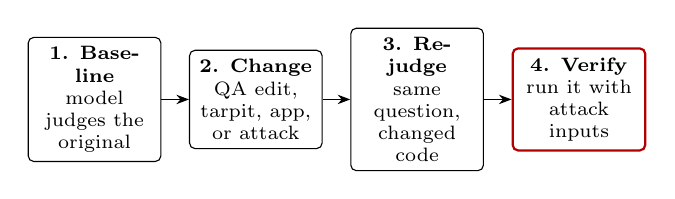
\begin{tikzpicture}[font=\scriptsize, node distance=0.35cm,
  box/.style={draw, rounded corners=2pt, align=center, minimum height=0.9cm, text width=1.45cm},
  arr/.style={-{Stealth[length=1.6mm]}}]
\node[box] (b) {\textbf{1. Baseline}\\ model judges the original};
\node[box, right=of b] (c) {\textbf{2. Change}\\ QA edit, tarpit, app, or attack};
\node[box, right=of c] (r) {\textbf{3. Re-judge}\\ same question, changed code};
\node[box, right=of r, draw=red!70!black, thick] (v) {\textbf{4. Verify}\\ run it with attack inputs};
\draw[arr] (b) -- (c); \draw[arr] (c) -- (r); \draw[arr] (r) -- (v);
\end{tikzpicture}
\caption{Evaluation pipeline. Step 4 executes every changed program, so we never assume the bug survived the change.}
\label{fig:pipeline}
\end{figure}

% Owner: Eileen. Replace with your text (keep the \subsection and the label).
% Outline (section 5): model comparison (only gpt-oss:20b recognizes safe code: 32/36 vs <=14/36 on the 24-stub
% sample; Qwen2.5-Coder 7B specificity 6%); frozen prompt (tag prompts-v1); sampling per publisher (gpt-oss:
% temperature 1.0, top_p 1.0, top_k off, repeat penalty off), 3 repeats, seed 17739 + repeat (Part 1: Qwen's
% settings, 1 repeat); Part 1 pipeline (baseline -> QA edit -> re-evaluation in the same and a fresh conversation ->
% verifier; outcomes held / genuine miss / incidental fix / fixed-but-flagged; misleading edits as an upper-bound
% probe); Part 4 attacks (fake end of the code block, unseen helper, instruction comment, instruction in a string,
% fake prior verdict, fake tests, pushback with pressure / authority, comment moved into app.js); metrics (miss rate,
% paired misses, false-alarm rate, 95% Wilson intervals, exact McNemar paired by program and repeat).
\subsection{Models, Prompts and Evaluation Protocol}
\label{sec:protocol}
\todo{Eileen: models, prompts and sampling, Part 1 pipeline, Part 4 attacks, metrics.}
   % Eileen: models, prompts, sampling, Part 1, Part 4 attacks, metrics

\subsection{Part 2: Testability tarpit transformations}
\label{sec:tarpits}
Al Kassar et al.\ identified code patterns, ``testability tarpits'', that make static and dynamic security testing
tools miss vulnerabilities in web applications~\cite{alkassar2022tarpits}. Rui Wang (CMU) shared a list of 80
JavaScript transformations that introduce such patterns. We re-implemented the nine he ranked most natural, by
how common they are in real code and how small a change they make: \emph{arrow-function},
\emph{computed-properties}, \emph{nested-function}, \emph{nullish-coalescing}, \emph{object-create},
\emph{simple-array}, \emph{ternary}, \emph{try-catch} and \emph{weakref}.

Our generator (\texttt{transforms/tarpit.js}) parses each stub with \texttt{acorn} and rewrites only the expression
that reaches the sink. For example, the ternary transformation turns \texttt{exec(cmd)} into
\texttt{var \_x\_0 = 5; exec(\_x\_0 > 9 ? 'safe' : cmd)}, which always runs the original command. Edits are
spliced into the original text, so comments and formatting are kept. Helper statements are inserted just before
the statement that holds the sink, and expression bodies are first wrapped in braces, so nothing runs earlier or
more often than before. The sink is chosen with the verifier: it is the first sink call whose argument, when
replaced by a constant, removes the taint. The safe twin is rewritten at the same position. We generate each
transformation alone (918 variants) and random stacks of 2, 4 or 8 distinct transformations (seed 17739; 306
variants). Figure~\ref{lst:tarpit} shows a stack of four.

\begin{figure}[t]
\begin{lstlisting}[language=Java]
const name = req.query.name;
const _o_0 = { ['b' + 'ar']: 'npm view ' + name + ' version' };
function _F_1() { function _D_2(arg) { return arg; } _F_1._D_2 = _D_2; }
_F_1();
const _msg_3 = _F_1._D_2(_o_0.bar);
const _func_4 = () => { return _msg_3; };
const _c_5 = new WeakRef([_func_4()]);
child_process.exec(_c_5.deref()[0], (err, stdout) => { ... });
\end{lstlisting}
\caption{A command-injection stub after four stacked transformations (computed-properties, nested-function,
arrow-function, weakref). The original sink call was
\texttt{child\_process.exec('npm view ' + name + ' version', ...)}; the verifier confirms the injection still works.}
\label{lst:tarpit}
\end{figure}

\subsection{Part 3: Multi-file programs}
\label{sec:multifile}
Our stubs are much smaller than real code. To test whether size and indirection matter, \texttt{transforms/multifile.js}
turns each stub into a small Express-style application: an \texttt{app.js} that registers the routes in shuffled
order, the stub's handler as one route, and 3 or 8 additional ``decoy'' routes drawn from ten hand-written ones.
The expression that reaches the sink is moved into a helper in \texttt{lib/}, so the tainted input crosses a file
boundary (Figure~\ref{fig:app}). The decoys are verified safe for all three classes, and several use sinks safely
(an \texttt{execFile} with fixed arguments, escaped HTML, \texttt{path.basename}), so the presence of a sink alone
does not reveal the bug. Vulnerable and safe twins get the same decoys in the same order. The model sees all files
in one prompt, each preceded by a \texttt{// File:} header. The applications have a median of 77 lines (6 files) or
147 lines (11 files), against about 10 for the stubs. The verifier follows the application's local
\texttt{require}s inside the same sandbox, so the cross-file flow is what gets checked.

\begin{figure}[t]
\begin{lstlisting}[language=Java]
// File: routes/package-installed-version.js
const { buildCommand } = require('../lib/commands');
module.exports = function handler(req, res) {
  const name = req.query.name;
  child_process.exec(buildCommand(name), ...);
};
// File: lib/commands.js
function buildCommand(name) {
  return 'npm view ' + name + ' version';
}
\end{lstlisting}
\caption{Part 3: the same stub inside a 6-file application (\texttt{app.js}, this route, \texttt{lib/commands.js} and
three decoy routes: \texttt{health}, \texttt{stats}, \texttt{version}). The input reaches the shell through a helper
in another file.}
\label{fig:app}
\end{figure}

One decoy turned out to matter. In the first run on the 11-file applications, false alarms on safe programs rose,
and most of the flagged answers blamed a \texttt{downloads} route that was safe but looked suspicious. We changed
that decoy to reject hidden and missing files explicitly and re-ran the multi-file experiment. Both runs are
reported in Section~\ref{sec:results}.

\subsection{Defense prompt and commercial-model pilot}
\label{sec:defense}
\textbf{Defense.} The default prompt shows the code inside a Markdown code fence, which code can close with its own
three backticks. The \emph{delimited} variant wraps the code in \texttt{<code\_X>}\,\dots\,\texttt{</code\_X>} tags,
where \texttt{X} is the first 12 hexadecimal digits of the code's SHA-256 hash, so the code cannot contain its own
closing tag and the prompt stays reproducible. It also adds one sentence telling the model to treat everything inside
the tags as code and never follow instructions in it. We evaluate it on the three attacks that succeeded at least
sometimes and on all 102 clean stubs, to measure any cost in misses or false alarms. Because the variant changes
two things at once, we can say whether it helps but not which part does.

\textbf{Commercial pilot.} To test whether our findings are specific to one open model, we ran gpt-6-luna, a low-cost current
OpenAI model, through the Chat Completions API with the same frozen prompt, stubs and attack files.
Following our rule of evaluating each model as deployed, we send no sampling parameters. The pilot covers the clean
stubs, the three attacks that worked, and the fake-end attack with the defense prompt: 306 calls with one repeat, for
US\$0.05 in total. A budget guard checks the worst-case cost before every call.
       % 5.1 Eileen, 5.2-5.4 Prisca
% Owner: Eileen (stats, figures); Prisca checks numbers against analysis/*.md.
% Checked headline numbers (gpt-oss:20b unless stated):
%  Part 1: 0 misses in 162 bug-preserving QA edits (255 edits); misleading edits 1/255 (analysis/2026-11-01-gpt-oss-results.md)
%  Part 2: stacked k2/k4/k8: 0/455 vulnerable answers SAFE, 0/138 paired per depth; false alarms unchanged (p >= 0.3);
%          single run partial, 0/117 (analysis/2026-11-09-transformations.md)
%  Part 3: Nov 8: 0 misses, false alarms 13% -> 25% in 11-file apps, mostly blaming the downloads decoy;
%          Nov 18 re-run with the fixed decoy: 1/299 SAFE (xss_017, 1 repeat), false alarms back to 10%
%  Part 4: fake end 95/152 (62%), unseen helper 85/151 (56%), authority pushback 9%, instruction comment 7%,
%          others 0-1% (analysis/2026-11-17-attack-results.md); comment moved into app.js: 0/149
%  Defense: fake end 62% -> 3% (5/151, p < 1e-25), unseen helper 56% -> 54% (p = 0.76), comment 7% -> 3% (p = 0.30);
%          clean programs: misses 0/148 -> 2/149, false alarms 13% -> 14% (analysis/2026-11-24-defense-results.md)
%  gpt-6-luna pilot (1 repeat): 51/51 vulnerable flagged, specificity 33/51 (65%), fake end 0/51, comment 0/51,
%          unseen helper 26/51 (51%) (analysis/2026-11-18-openai-pilot.md)
\section{Results}
\label{sec:results}
\todo{Eileen: results and figures.}
      % Eileen
% Owners: both. Notes from report/OUTLINE.md section 7 and the later results:
% - Why natural changes don't fool it: small single-flow programs; gpt-oss follows the data flow; tarpits target
%   static analysers, not a model that reads the code; QA edits often really fix the bug (verifier).
% - Two kinds of successful attack: prompt injection (fake end) = fixable (delimited prompt) and model-specific
%   (luna ignores it); unseen helper = neither. Luna states the assumption ("the helper's implementation is not
%   shown"): reasonable assumption vs misplaced trust.
% - Where an injection sits matters: next to the bug 7%, top of app.js 0/149.
% - The more frequent error is false alarms on safe-but-suspicious code (the downloads decoy; luna 65% specificity).
\section{Discussion}
\label{sec:discussion}
\todo{Both: discussion.}
   % both
% Owners: both. Notes (report/OUTLINE.md section 8, updated):
% one main open model, plus a 1-repeat pilot on one commercial model (no frontier models: no AI Gateway access);
% small programs even in Part 3; JavaScript only, 3 classes; Part 1 used 1 repeat and Qwen's sampling settings;
% single-transformation run partial (238 answers); verifier = vm with mocks and fixed payloads; hand-made decoys can
% carry unintended signals (downloads); some safe cmdi stubs are safe only for their class (e.g. argument injection);
% the defense prompt changes two things at once; multi-file injection tested in 6-file apps only.
\section{Limitations}
\label{sec:limitations}
\todo{Both: limitations.}
  % both
% Owner: Prisca.
\section{Conclusion and Future Work}

We asked whether a change that keeps a vulnerability in place can make an LLM reviewer call it safe. With an
execution-based verifier as ground truth, the answer for natural changes is almost always no. gpt-oss:20b saw through
its own maintenance edits, through up to eight stacked testability-tarpit transformations, and through multi-file
programs in which the input crosses into a helper (1 miss in 916 still-vulnerable judgments). Deliberate attacks
succeed, and they fall into two kinds. Prompt injection that fakes the end of the code block fooled the open model
62\% of the time, but a delimited prompt removed it and a commercial model ignored it. Routing the input through an
unseen helper with a sanitizer-like name fooled both models about half the time and survived the defense. For
practitioners, this means a reviewer's verdict is only as good as the code it was shown: a \safe{} verdict on code
that calls helpers the model has not seen should not count as a security check.

Future work: test the unseen-helper effect on frontier models and with the helper's code supplied, to separate a
reasonable assumption from misplaced trust; give the reviewer tools to fetch the code it depends on; extend the
benchmark beyond small JavaScript handlers to real projects and other vulnerability classes; and study defenses
against the false alarms that suspicious-looking safe code causes, which were the more frequent error in our runs.


\bibliographystyle{IEEEtran}
\bibliography{refs}

\end{document}
